\documentclass[]{article}
\usepackage{lmodern}
\usepackage{amssymb,amsmath}
\usepackage{ifxetex,ifluatex}
\usepackage{fixltx2e} % provides \textsubscript
\ifnum 0\ifxetex 1\fi\ifluatex 1\fi=0 % if pdftex
  \usepackage[T1]{fontenc}
  \usepackage[utf8]{inputenc}
\else % if luatex or xelatex
  \ifxetex
    \usepackage{mathspec}
  \else
    \usepackage{fontspec}
  \fi
  \defaultfontfeatures{Ligatures=TeX,Scale=MatchLowercase}
\fi
% use upquote if available, for straight quotes in verbatim environments
\IfFileExists{upquote.sty}{\usepackage{upquote}}{}
% use microtype if available
\IfFileExists{microtype.sty}{%
\usepackage{microtype}
\UseMicrotypeSet[protrusion]{basicmath} % disable protrusion for tt fonts
}{}
\usepackage[margin=1in]{geometry}
\usepackage{hyperref}
\PassOptionsToPackage{usenames,dvipsnames}{color} % color is loaded by hyperref
\hypersetup{unicode=true,
            pdftitle={Analysis of proportion of human pathogens for different phylums from JGI IMG database},
            pdfauthor={Miroshnikova Anastasia},
            colorlinks=true,
            linkcolor=Maroon,
            citecolor=Blue,
            urlcolor=blue,
            breaklinks=true}
\urlstyle{same}  % don't use monospace font for urls
\usepackage{graphicx,grffile}
\makeatletter
\def\maxwidth{\ifdim\Gin@nat@width>\linewidth\linewidth\else\Gin@nat@width\fi}
\def\maxheight{\ifdim\Gin@nat@height>\textheight\textheight\else\Gin@nat@height\fi}
\makeatother
% Scale images if necessary, so that they will not overflow the page
% margins by default, and it is still possible to overwrite the defaults
% using explicit options in \includegraphics[width, height, ...]{}
\setkeys{Gin}{width=\maxwidth,height=\maxheight,keepaspectratio}
\IfFileExists{parskip.sty}{%
\usepackage{parskip}
}{% else
\setlength{\parindent}{0pt}
\setlength{\parskip}{6pt plus 2pt minus 1pt}
}
\setlength{\emergencystretch}{3em}  % prevent overfull lines
\providecommand{\tightlist}{%
  \setlength{\itemsep}{0pt}\setlength{\parskip}{0pt}}
\setcounter{secnumdepth}{0}
% Redefines (sub)paragraphs to behave more like sections
\ifx\paragraph\undefined\else
\let\oldparagraph\paragraph
\renewcommand{\paragraph}[1]{\oldparagraph{#1}\mbox{}}
\fi
\ifx\subparagraph\undefined\else
\let\oldsubparagraph\subparagraph
\renewcommand{\subparagraph}[1]{\oldsubparagraph{#1}\mbox{}}
\fi

%%% Use protect on footnotes to avoid problems with footnotes in titles
\let\rmarkdownfootnote\footnote%
\def\footnote{\protect\rmarkdownfootnote}

%%% Change title format to be more compact
\usepackage{titling}

% Create subtitle command for use in maketitle
\newcommand{\subtitle}[1]{
  \posttitle{
    \begin{center}\large#1\end{center}
    }
}

\setlength{\droptitle}{-2em}
  \title{Analysis of proportion of human pathogens for different phylums from JGI
IMG database}
  \pretitle{\vspace{\droptitle}\centering\huge}
  \posttitle{\par}
  \author{Miroshnikova Anastasia}
  \preauthor{\centering\large\emph}
  \postauthor{\par}
  \predate{\centering\large\emph}
  \postdate{\par}
  \date{8 August 2017}


\begin{document}
\maketitle

{
\hypersetup{linkcolor=black}
\setcounter{tocdepth}{2}
\tableofcontents
}
\subsection{Introduction}\label{introduction}

The study to be published here is part of a student project which took
place at
\href{http://bioinformaticsinstitute.ru/summer2017}{Bioinformatics
Institute Summer School - 2017}.The data set used in the study is
downloaded from \href{https://img.jgi.doe.gov/cgi-bin/m/main.cgi}{JGI
IMG database}\footnote{Here is the
  \href{https://raw.githubusercontent.com/Miffka/RAnalysis2FinalTask/master/IMG_all-more\%2Bpathog.xls}{direct
  link} to data download.} with multiple filters. The original study was
based on Deneke and Renard (2017).

The original data set contains 9563 records about sequenced bacterial
genomes, but only 1858 possess information about organism phenotype. The
analyzed bacteria were presented by 368 species, which belonged to one
of 77 families. These families belonged to one of theese phylums:

\begin{verbatim}
##  [1] "Firmicutes"      "Proteobacteria"  "Actinobacteria" 
##  [4] "Tenericutes"     "Chlamydiae"      "Bacteroidetes"  
##  [7] "Fusobacteria"    "Spirochaetes"    "Synergistetes"  
## [10] "Cyanobacteria"   "Deferribacteres"
\end{verbatim}

\subsection{Hypothesis}\label{hypothesis}

We were interested in obtaining reliable and self-consistent sequencing
data, so we decided to find out whether there is a statistically
significant difference in proportion of sequenced pathogens in different
phylums of bacteria. For these purpose we used \textbf{R} (version
3.4.1) and two appropriate statistical tests called \emph{Pearson's
Chi-square}: \[X^2 = \sum_{}{}\frac{(O - E)^2}{E} \] and \emph{Fisher's
exact test}:
\[P_{cutoff} = \frac{(R_1!R_2!...R_m!)(C_1!C_2!...C_n!)}{N!\prod_{ij}^{}a_{ij}} \]

Our zero hypothesis is that proportion of sequenced pathogens over total
sequenced samples of the phylum is the same for all phylums.

The workflow is as follows:

\begin{enumerate}
\def\labelenumi{\arabic{enumi}.}
\tightlist
\item
  Read file
\item
  Prepare data for analysis
\item
  Run chi-square test and Fisher's exact test for all appropriate
  phylums and obtain p-value
\item
  Support the evidence with

  \begin{itemize}
  \tightlist
  \item
    a table of results;
  \item
    a plot that could help demonstrate them.
  \end{itemize}
\end{enumerate}

\subsection{Analysis}\label{analysis}

Because of database format, there are 71 different types of phenotype.
That's why before the analysis we added a new variable with only two
phenotype levels - either ``Pathogen'' or ``Non-Pathogen''.

It turned out that for some phylums there was not enough observations
even for Fisher's exact test (less than 8 for whole phylum). These
phylums, i.e.~Cyanobacteria, Deferribacteres, Synergistetes were
excluded from the analysis. For the other phylums there was no data on
sequenced non-pathogens, so they were also excluded from analysis
(Chlamydiae, Spirochaetes, Tenericutes). The final data to be analyzed
by Fisher's exact test were as follows:

\begin{verbatim}
##                 
##                  Non-Pathogen Pathogen
##   Actinobacteria           58      107
##   Bacteroidetes            22       29
##   Firmicutes               86      740
##   Fusobacteria              3       10
##   Proteobacteria          146      554
\end{verbatim}

For chi-sqared test the phylum Fusobacteria was excluded.

So structure of our data was as follows:

\begin{figure}[htbp]
\centering
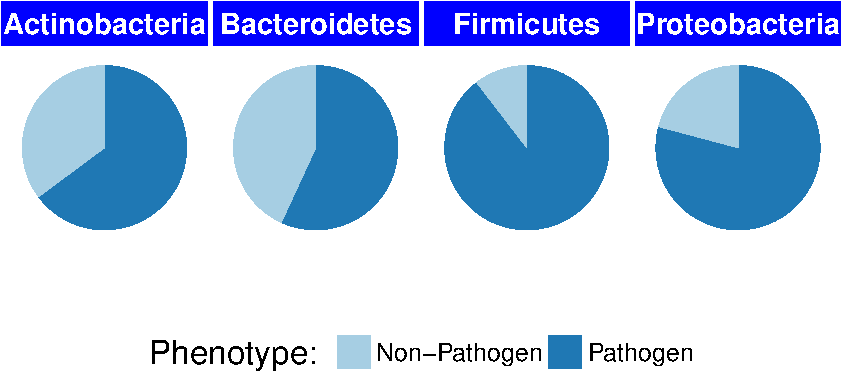
\includegraphics{303_finaltask_files/figure-latex/primary_graphics-1.pdf}
\caption{Relative distribution of phylums in pathogenic and
non-pahtogenic sequenced samples}
\end{figure}

The p-value for the tests were \(3.48\times 10^{-18}\) for Fisher's
exact test and \(1.234\times 10^{-19}\) for chi-squared test
(\(1.127\times 10^{-18}\) for the same data). This let us to say that
proportion of pathogens is different for at least one phylum.

For chi-squared test a matrix of residuals was

\begin{verbatim}
##                 
##                  Non-Pathogen Pathogen
##   Actinobacteria         5.23    -2.44
##   Bacteroidetes          4.26    -1.99
##   Firmicutes            -5.09     2.38
##   Proteobacteria         1.84    -0.86
\end{verbatim}

\begin{figure}[htbp]
\centering
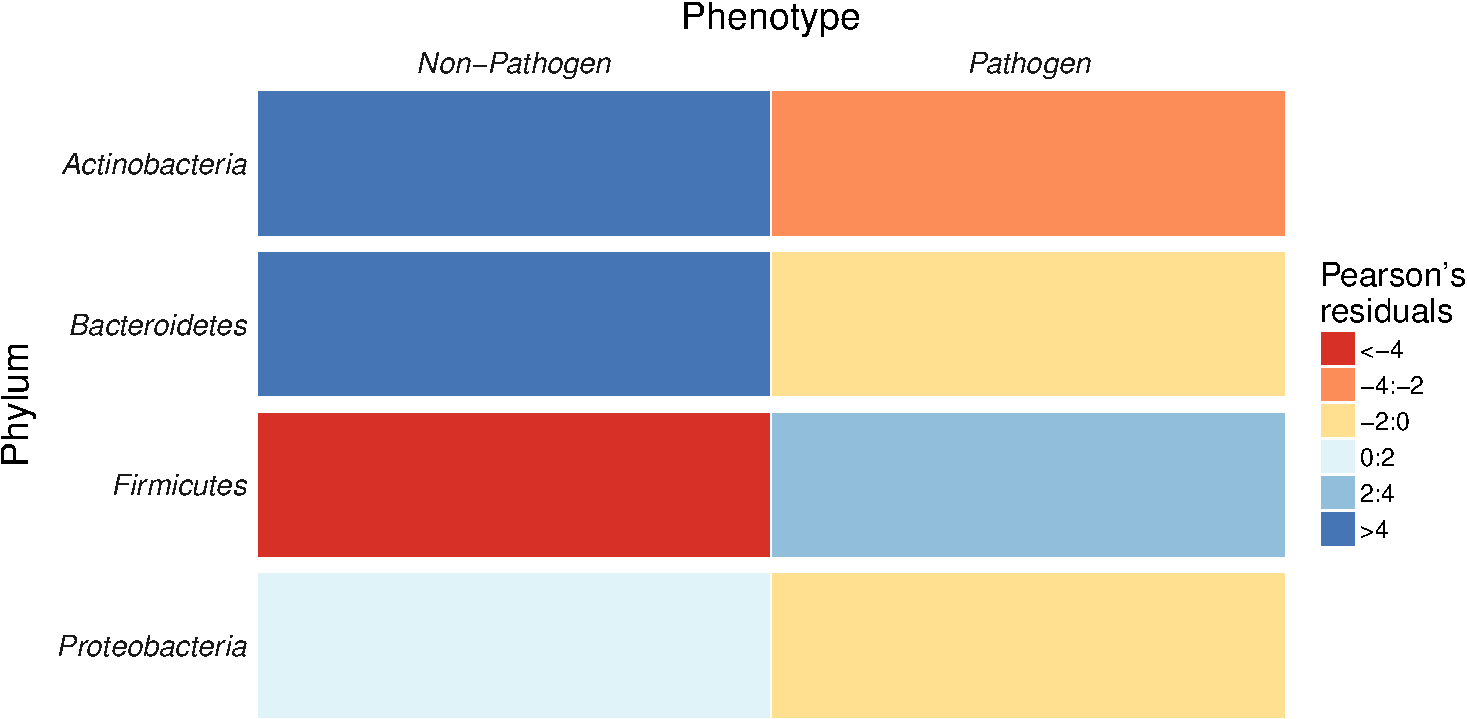
\includegraphics{303_finaltask_files/figure-latex/vizualization2-1.pdf}
\caption{Pearson's residuals for different phylums}
\end{figure}

As we see, the proportion of sequenced non-pathogenic members of
Actinobacteria and Bacteroidetes phylums is far more than expected, and
proportion of non-pathogenic members of Firmicutes phylum is less than
expected.

\subsection{Conclusion}\label{conclusion}

Our hypothesis of non-uniform distribution of sequenced pathogens over
different phylums in the data base of interest was proven to be valid.

\subsection{Acknowledgements}\label{acknowledgements}

Author is very grateful to the Organizing Commitee of
\textbf{Bioinformatics Institute Summer School - 2017} for letting a
chance to obtain such interesting data.

\subsection*{Bibliography}\label{bibliography}
\addcontentsline{toc}{subsection}{Bibliography}

\hypertarget{refs}{}
\hypertarget{ref-PaPrBaG}{}
Deneke, Rentzsch, C., and B.Y. Renard. 2017. ``PaPrBaG: A Machine
Learning Approach for the Detection of Novel Pathogens from Ngs Data.''
\emph{Nature Scientific Reports} 7 (39194).
doi:\href{https://doi.org/10.1038/srep39194}{10.1038/srep39194}.


\end{document}
